% Generated by plsimcount.pffigure -- do not edit; regenerate instead.
% figure: A-com-by-order -- Suzuki formulas of each order, r from: Commutator bound (2018)
% source: results/pf-thesis/results.json
% metric=cnot gatebase=cz merged
% seed=1 t=n template=simcount synth=pygridsynth
% git_commit=c237fe494a6c663dd73df63b2b3fbb5e397a506e git_dirty=False
% source_sha256=6e8b2641428f03f62fe1dfd44b32f3373e9b382199e065d6a7d7340c7875a117
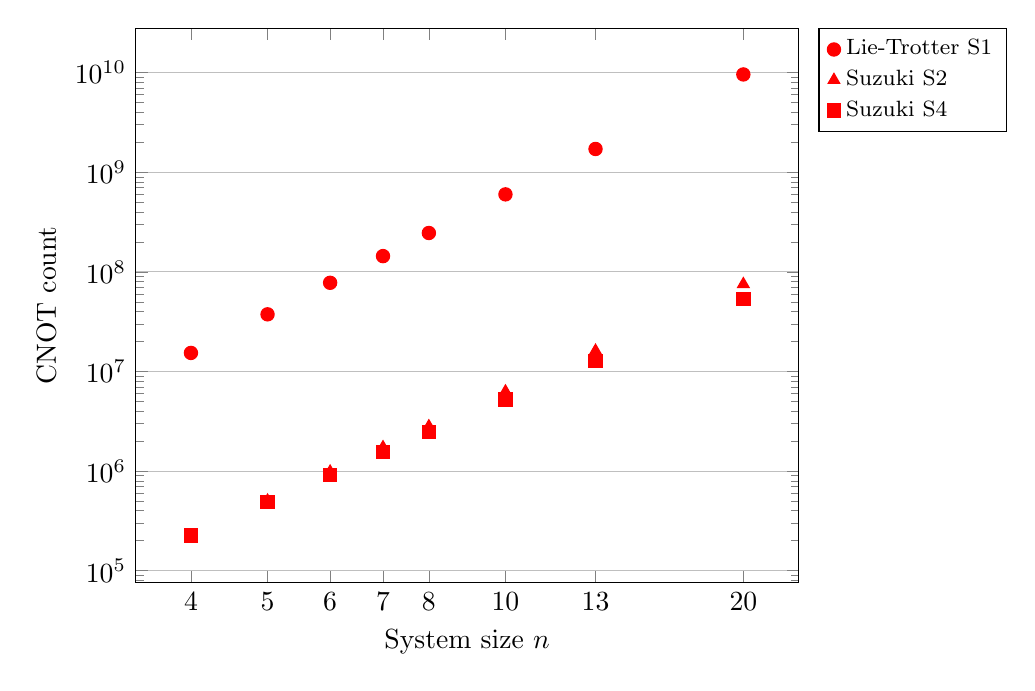
\begin{tikzpicture}
  \begin{loglogaxis}[
    width=10cm,
    xlabel={System size $n$},
    ylabel={CNOT count},
    xtick={4,5,6,7,8,10,13,20},
    xticklabels={4,5,6,7,8,10,13,20},
    ymajorgrids=true,
    legend pos=outer north east,
    legend cell align=left,
    legend style={font=\footnotesize},
  ]
    \addplot[only marks, red, mark=*, mark size=2.4pt, mark options={solid, fill=red}] coordinates {
      (4,15363288)
      (5,37508010)
      (6,77776596)
      (7,144090744)
      (8,245812464)
      (10,600127980)
      (13,1714025586)
      (20,9602047680)
    };
    \addlegendentry{Lie-Trotter S1}
    \addplot[only marks, red, mark=triangle*, mark size=2.4pt, mark options={solid, fill=red}] coordinates {
      (4,220120)
      (5,505500)
      (6,988260)
      (7,1734180)
      (8,2815200)
      (10,6299800)
      (13,16163550)
      (20,75392000)
    };
    \addlegendentry{Suzuki S2}
    \addplot[only marks, red, mark=square*, mark size=2.4pt, mark options={solid, fill=red}] coordinates {
      (4,226632)
      (5,490350)
      (6,918288)
      (7,1557612)
      (8,2457504)
      (10,5243700)
      (13,12704328)
      (20,53642400)
    };
    \addlegendentry{Suzuki S4}
  \end{loglogaxis}
\end{tikzpicture}
